\documentclass{article}

% If you're new to LaTeX, here's some short tutorials:
% https://www.overleaf.com/learn/latex/Learn_LaTeX_in_30_minutes
% https://en.wikibooks.org/wiki/LaTeX/Basics

% Formatting
\usepackage[utf8]{inputenc}
\usepackage[margin=1in]{geometry}
\usepackage[titletoc,title]{appendix}

% Math
% https://www.overleaf.com/learn/latex/Mathematical_expressions
% https://en.wikibooks.org/wiki/LaTeX/Mathematics
\usepackage{amsmath,amsfonts,amssymb,mathtools}

% Images
% https://www.overleaf.com/learn/latex/Inserting_Images
% https://en.wikibooks.org/wiki/LaTeX/Floats,_Figures_and_Captions
\usepackage{graphicx,float}
\usepackage{caption}
\usepackage{subcaption}

% Tables
% https://www.overleaf.com/learn/latex/Tables
% https://en.wikibooks.org/wiki/LaTeX/Tables

% Algorithms
% https://www.overleaf.com/learn/latex/algorithms
% https://en.wikibooks.org/wiki/LaTeX/Algorithms
\usepackage[ruled,vlined]{algorithm2e}
\usepackage{algorithmic}

% Code syntax highlighting
% https://www.overleaf.com/learn/latex/Code_Highlighting_with_minted
\usepackage{minted}
\usemintedstyle{borland}
\usepackage{listings}


% References
% https://www.overleaf.com/learn/latex/Bibliography_management_in_LaTeX
% https://en.wikibooks.org/wiki/LaTeX/Bibliography_Management
\usepackage{biblatex}
\addbibresource{references.bib}

% Title content
\title{AMATH 482 Homework 5}
\author{Rishabh Verma}
\date{March 17th, 2021}

\begin{document}

\maketitle

% Abstract
\begin{abstract}
	Sequential frames of a video can be regarded as a transformation of the previous. In the process of Dynamic Mode Decomposition, this transformation is assumed to be linear and decomposed. Out of the resulting components, the constant-order ones can be used to isolate the background of the video. The background is then subtracted from the original video to successfully isolate the foreground.
\end{abstract}

% Introduction and Overview
\section{Introduction and Overview}
Background subtraction is the process of isolating the foreground and background from a video. The task of this lab is to carry out background separation on two videos, both of which are filmed from a fairly stable camera perspective. 

Both videos have a resolution of 540x960 and are 6 seconds long. They are both screen-recordings of a device displaying the video, and so are re-sampled to be 60 frames per second, though the fact that each frame is accompanied by two or three duplicate frames suggests that the original source material is closer to 24 frames per second. All duplicate frames are later stripped anyway.

The subject of the first video is a group of racecars on a racetrack. The racecars are prominent objects which fill up a good portion of the screen, and their color stands out from the background. 

The subject of the second video is a skiier descending down a slope. This video is filmed from afar, and the skiier is very small. The skiier is wearing dark clothing against a white slope, but because the skiier is so small and the foreground includes the snow kicked up in the skiier's wake, of similar color to the background snow, this video presents a more difficult challenge for background subtraction.

%  Theoretical Background
\section{Theoretical Background}
\subsection{The Koopman operator}
Consider a set of numerical observations evenly spaced in time, represented as column vectors $\mathbf{x}_1,\mathbf{x}_2,...,\mathbf{x}_n$. Let us make the assumption that the transition from one observation to the next is a constant linear function. It can then be represented by the matrix $A$, which satisfies

\begin{equation}
	\mathbf{x}_{j+1} = A\mathbf{x}_j
	\label{eqn:koopman}
\end{equation}

for all applicable $j$. This treats the state space like a solution to an unknown linear ODE, where transitions between states involve linear operations on the states. 

\subsection{Dynamic Mode Decomposition}
Dynamic Mode Decomposition is a method of approximating a Koopman operator for our data. Suppose our numerical observations form the columns of a data matrix $X$. Furthermore, define the matrices $X_1,X_2$ by deleting the last and first column of $X$ respectively. 

\begin{equation}
	X_1 := \begin{bmatrix}
		\mathbf{x}_1& \mathbf{x}_2 &... & \mathbf{x}_{n-1}
	\end{bmatrix}
\end{equation}

\begin{equation}
	X_2 := \begin{bmatrix}
		\mathbf{x}_2 & \mathbf{x}_3 & ... & \mathbf{x}_n
	\end{bmatrix}
\end{equation}

These matrices are almost related through left-multiplication by $A$, as is leveraged in Equation~\ref{eqn:dmd_koopman}, where $\mathbf{r}$ is the error of the last column, and $e^\top_{n-1}$ is the standard basis vector to put these error vector in the right place for matrix addition.

\begin{equation}
	X_2 = AX_1 + \mathbf{r}e^\top_{n-1}
	\label{eqn:dmd_koopman}
\end{equation}

We can't solve for $A$ in closed form, but we can compute a matrix similar to it and indirectly obtain $A$'s eigenvalues and eigenvectors, telling us enough we need to know about $A$. Compute the reduced Singular Value Decomposition of $X_1 = U\Sigma V^*$ where $\Sigma$ is square and $V^*$ only contains the row-space right singular vectors, and substitute this into Equation~\ref{eqn:dmd_koopman}. We want to choose $A$ such that the matrix $X_2$ is now expressed as a linear combination only of the columns of $U$, and that the residual vector is orthogonal to $U^*$. Under this assumption, we can left-multiply Equation~\ref{eqn:dmd_koopman} by $U^*$, right-multiply by $V$ and simplify. 

\begin{equation}
	\begin{split}
		X_2 &=AU\Sigma V^* + \mathbf{r}e^\top_{n-1}\\
		U^*X_2&=U^*AU\Sigma V^*\\
	\tilde{S} := U^*X_2V \Sigma^{-1}&=U^*AU
	\end{split}
	\label{eqn:DMD}
\end{equation}

The algebra expressed in Equation Set~\ref{eqn:DMD} provides a matrix $\tilde{S}$ similar to $A$. An eigenvalue/eigenvector pair of $\tilde{S}=U^*AU$,  represented as $\tilde{S}\mathbf{v}=\lambda \mathbf{v}$, will also satisfy Equation Set~\ref{eqn:eigen}, so then $U\mathbf{v}$ is an eigenvector of $A$ with eigenvalue $\lambda$.

\begin{equation}
	\begin{split}
	U^*AU\mathbf{v} &= \lambda \mathbf{v}\\
	AU\mathbf{v}&=U\lambda \mathbf{v}\\
	A(U\mathbf{v})&=\lambda(U\mathbf{v})
	\end{split}
	\label{eqn:eigen}
\end{equation}

We can store the eigenvectors of $A$ as a matrix product $\Phi = \begin{bmatrix}
	U\begin{bmatrix}
		\mathbf{y}_1 & \mathbf{y}_2 & ... & \mathbf{y}_K
	\end{bmatrix}
\end{bmatrix}$ where $K$ is the rank of $A$, and equivalently the number of eigenvectors outside the nullspace.

For each eigenvalue $\mu_k$, let $\omega_k = \log(\mu_k)/\Delta t$. Then our DMD approximation for the columns of $X$ in terms of $\mathbf{x}_1$ can be represented as a linear combination of exponentials in Equation~\ref{eqn:approximation}

\begin{equation}
	\mathbf{x}_{DMD}(t) = \sum_{k=1}^K b_k \Phi_ke^{\omega_k t}
	\label{eqn:approximation}
\end{equation}

The coefficients $\mathbf{b}$ are constant, and when evaluating $\mathbf{x}_{DMD}(0) = \sum_{k=1}^K b_k \Phi_k = \Phi \mathbf{b}$ (where $\Phi_k$ is the $k$-th column of $\Phi$), I can solve for $\mathbf{b}$ in terms of $\mathbf{x}_1$ and the pseudo-inverse of $\Phi$.

\subsection{Background subtraction}

Each column of $\mathbf{x}_i$ can now be represented as a linear combination of the $K$ DMD modes, which are themselves exponential functions. An exponential function $e^{\omega_kt}$ can represented exponential growth, decay, oscillation, or a constant depending on the value of $\omega_k$. A constant-valued exponential function $e^{\omega_kt}$ would only come from an $\omega_k$ equal to or close to zero, which itself comes from an eigenvalue $\mu_k$ equal to or close to $1$. Such values characterize a component of an image which is constant throughout the matrix; such components can be effectively regarded as "backgrounds", capturing the portion of a video which is primarily still. 


\begin{algorithm}[]
	\KwIn{Data matrix $X$, evenly-spaced time evaluations $\mathbf{t}$ starting from $t=0$}
	\begin{algorithmic}
		\STATE{Set $X_1,X_2$ by deleting the last or first column of $X$ respectively.}
		\STATE{Compute the reduced SVD $X_1 = U\Sigma V^\top$}
		\STATE{Compute $\tilde{S} = U^*X_2V\Sigma^{-1}$}
		\STATE{Compute the diagonalization $\tilde{S} = QDQ^{-1}$}
		\STATE{Logarithmize the eigenvalues and store in $\omega = \text{log}(\text{diag}(D))\cdot \dfrac{1}{\Delta t}$}
		\STATE{Compute the eigenvectors of $A$ and store in $\Phi = UQ$}
		\STATE{Solve $\Phi b = \mathbf{x}_1$ using the pseudo-inverse of $\Phi$}
		\STATE{Initialize an empty $K \times n$ matrix $M$ for the modes}
		\FOR{all $t_i$}
		\STATE{Store the point-wise product of $\mathbf{b},\omega$ as the $i$-th row in $M$}
		\ENDFOR{}
		\RETURN{$M,\omega, \Phi$}
	\end{algorithmic}
	\label{alg:dmd}
	\caption{Dynamic Mode Decomposition}
\end{algorithm}


% Algorithm Implementation and Development
\section{Algorithm Implementation and Development}

All data should be evenly-spaced in time. The given video data has many sequential duplicate frames, and these were stripped before forming the data matrix $X$.

\begin{algorithm}[!t]
	\KwIn{Data matrix $X$, $M,\omega,\Phi$ from Alg.~\ref{alg:dmd}, threshold $\epsilon > 0$}
	\begin{algorithmic}
		\STATE{Initialize the background matrix $B$ as an empty $l\times n-1$ matrix where $X\in\mathbb{R}^{l\times n}$}
		\FOR{all $\omega_k$ with modulus less than $\epsilon$}
		\STATE{Compute the product $P$ of the $j$-th column of $\Phi$ and the $j$-th row of $M$}
		\STATE{Update $B$ to $B+P$}
		\ENDFOR{}
		\STATE{Compute $F = X - |B|$ where $|\cdot|$ denotes the modulus of each element}
		\RETURN{the foreground/background matrices $F,B$}
	\end{algorithmic}
	\label{alg:background}
	\caption{Background subtraction}
\end{algorithm}
	
Proper choice of threshold will depend on how close or how far the logarithmized eigenvalues $\omega$ are to $0$. A threshold of $\epsilon = 1\times 10^{-1}$ was found to be effective for both data samples in this paper. See Figure~\ref{fig:fig1} and Figure~\ref{fig:fig2}.

% Computational Results
\section{Computational Results}

For each video, the eigenvalues of $A$, $\mu$, are mostly close to the unit circle. This suggests that each transition according to Equation~\ref{eqn:koopman} does not change the overall spectral power of an image very much. The only eigenvalues used to construct the background image are the ones that are closest to one, identified by the ones whose logarithm is closest to zero. There is one such mode in the racing video, and there are two such modes in the skiing video, though they appear as only one mode in Figure~\ref{fig:fig2}

\begin{figure}
	\centering
	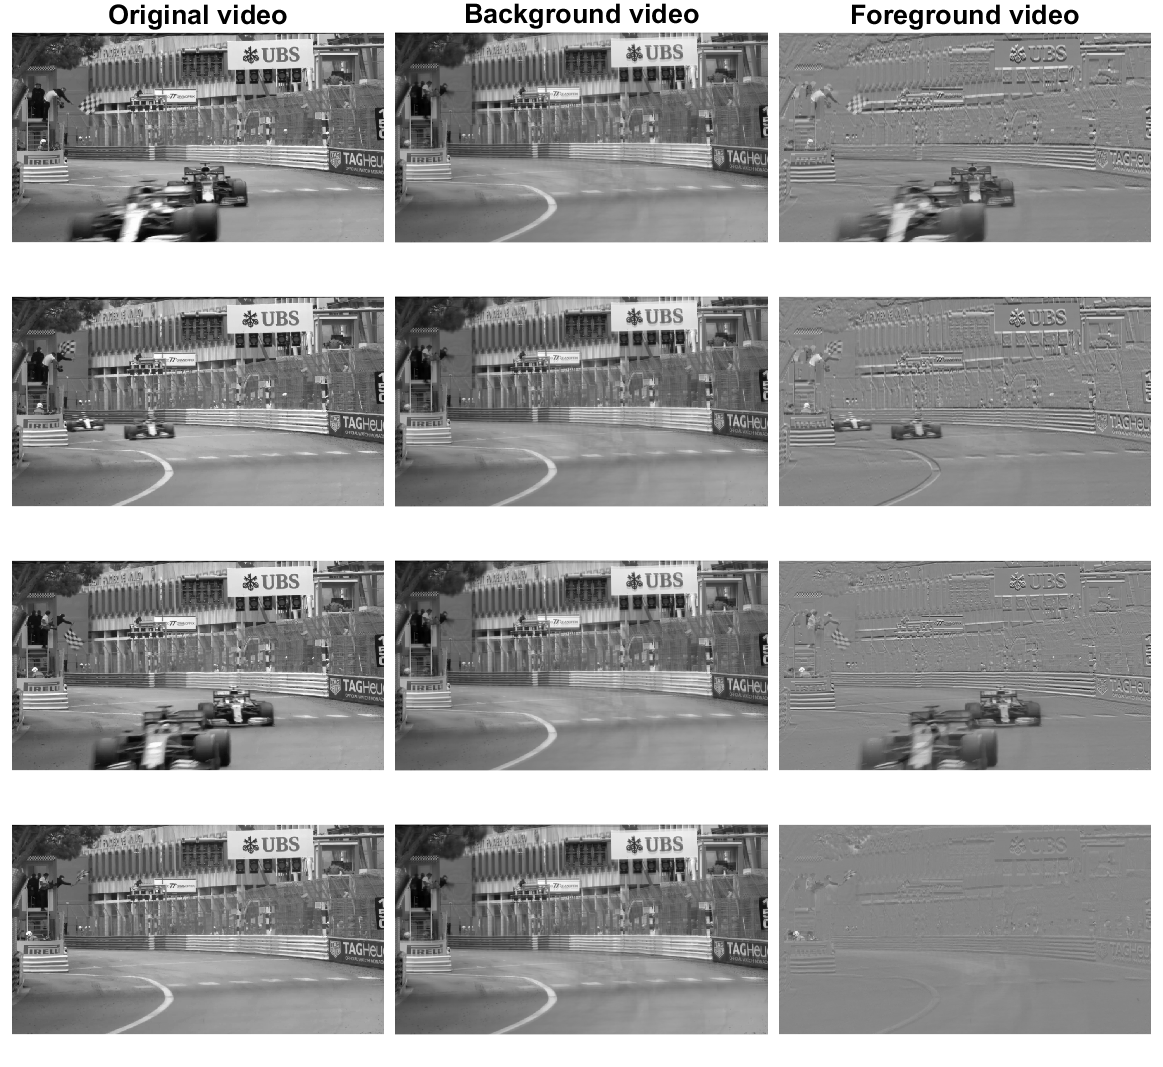
\includegraphics[scale=0.7]{figs/monte_carlo_result}
	\caption{Four frames from the racing video}
	\label{fig:fig3}
\end{figure}


\begin{figure}
	\centering
	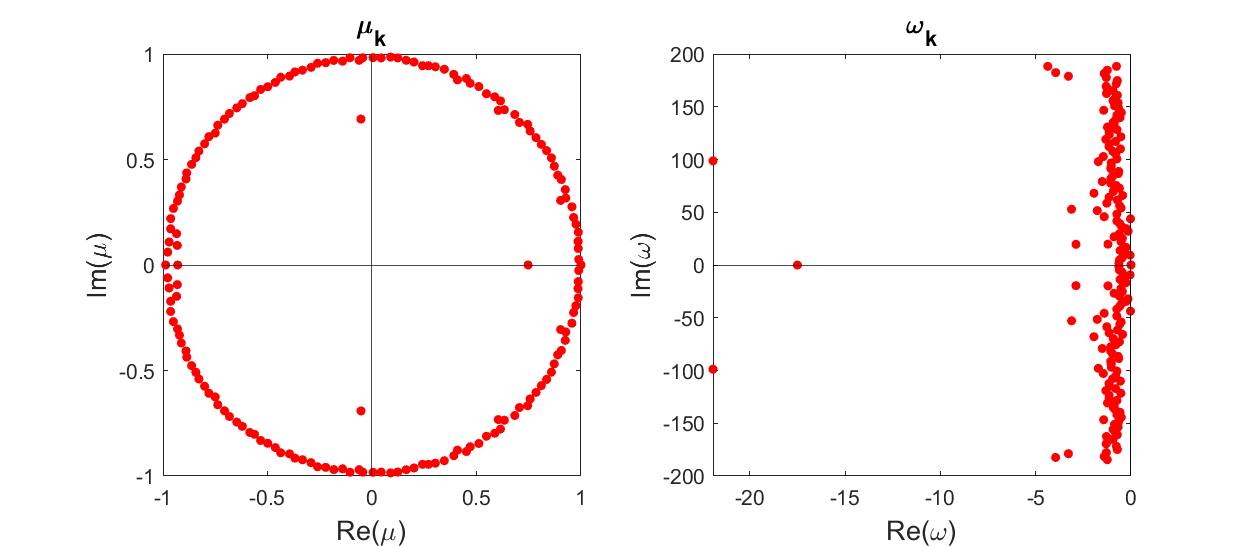
\includegraphics[scale=0.7]{figs/monte_carlo_eigen}
	\caption{Distribution of eigenvalues and their logarithm for racing video}
	\label{fig:fig1}
\end{figure}


\begin{figure}
	\centering
	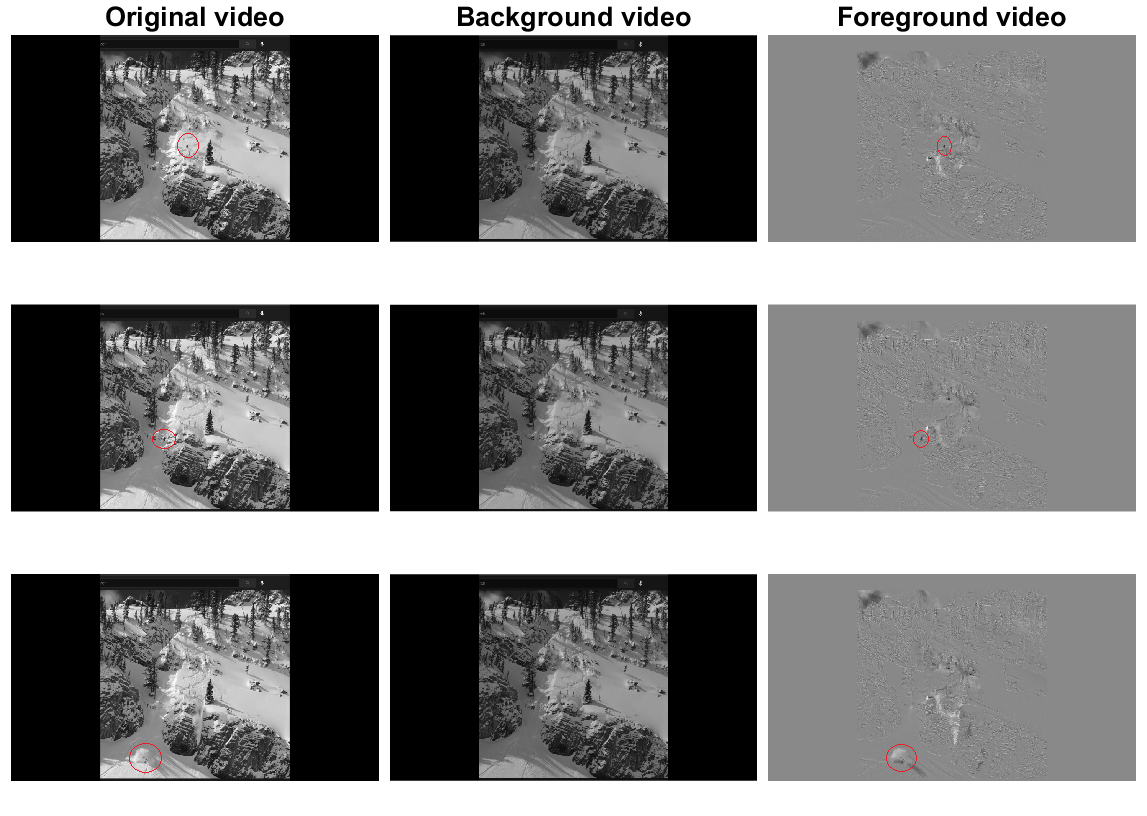
\includegraphics[scale=0.8]{figs/ski_drop_result}
	\caption{Three frames from the skiing video (location circled)}
	\label{fig:fig4}
\end{figure}

\begin{figure}
	\centering
	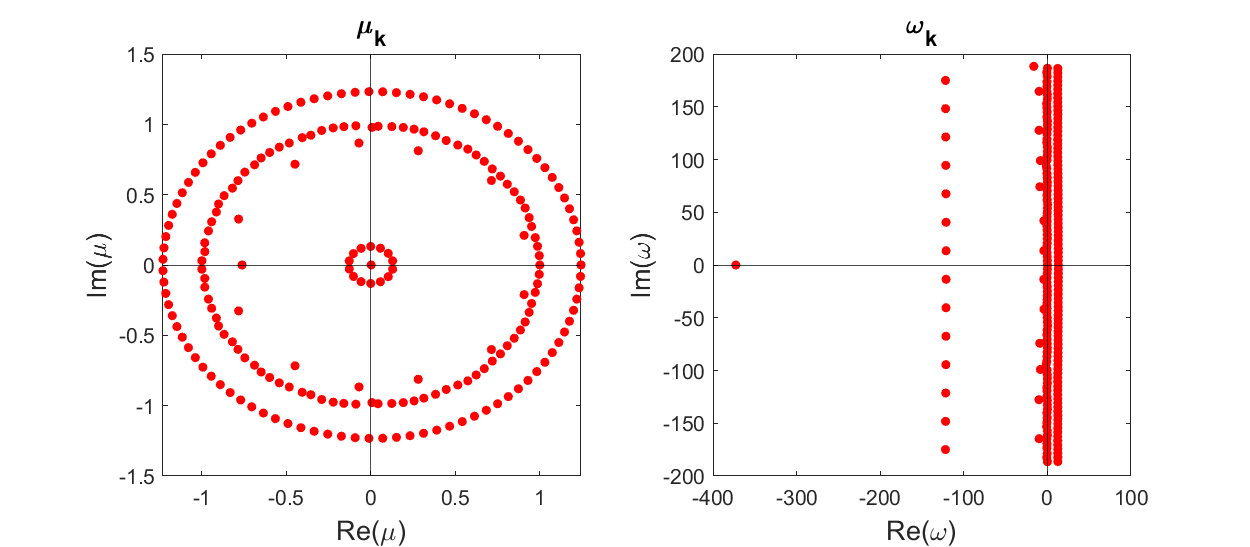
\includegraphics[scale=0.7]{figs/ski_drop_eigen}
	\caption{Distribution of eigenvalues and their logarithm for skiing video}
	\label{fig:fig2}
\end{figure}

% Summary and Conclusions

\section{Summary and Conclusions}

Dynamic Mode Decomposition is successful at isolating the background in both the skiing and the racecar videos. Subtracting this background image from the original video yields the foreground well in both the racing video and the skiing video. 

The skiing video is intended to be the "stress test" for background subtraction, and while some features of the background are retained in the foreground video, the true foreground is at least included in the right places. In Figure~\ref{fig:fig4}, the location of the skiier is circled in red in both the original and the foreground video. The image in the third row contains a large snow plume, which is correctly identified in the foreground.

In conclusion, the "foreground video" retains some features of the background which make the result imperfect for an application like CGI where visual reconstruction needs to be perfect. However, this could be used as one step in a sequence of algorithms to isolate the foreground with more photo processing techniques, or in a computer vision sequence of operations where minor visual noise can be thresholded.

% References
\printbibliography
\newpage 
% Appendices
\begin{appendices}

% MATLAB Functions
\section{MATLAB Functions}

\begin{itemize}
	\item \texttt{[U,S,V] = svd(X, 'econ')} gives the reduced SVD of $X$.
	
	\item \texttt{A \ b}, where system $A$ is underdetermined, solves the pseudo-inverse.
	
    \item \texttt{subplot\_tight()} by Nikolay S., Retrieved from MATLAB File Exchange. Allows for easy re-spacing of subplots in figures~\ref{fig:fig1},~\ref{fig:fig3}.
\end{itemize}

% MATLAB Codes
\section{MATLAB Code}

\subsection{main.m}
\inputminted{matlab}{main.m}

\subsection{subplot\_tight.m, by Nikolay S.}
\inputminted{matlab}{subplot_tight.m}
\end{appendices}
\end{document}